\documentclass[10pt,letterpaper]{article}
\usepackage[utf8]{inputenc}
\usepackage[spanish]{babel}
\usepackage{amsmath}
\usepackage{amsfonts}
\usepackage{amssymb}
\usepackage{graphicx}
\usepackage{ifthen}
\usepackage{forloop}
\usepackage{subfiles}
\usepackage{setspace}
\usepackage{listings}
\usepackage{xcolor}
\usepackage{lstlinebgrd}
\usepackage{float}
\usepackage{hyperref}

\hypersetup{
    colorlinks=true,
    linkcolor=blue,
    filecolor=magenta,      
    urlcolor=cyan,
}

\urlstyle{same}

\usepackage[left=2cm,right=2cm,top=2cm,bottom=2cm]{geometry}
\thispagestyle{empty}

%--! Codigo por defecto (no tocar si no sabes)

%\renewcommand{\familydefault}{\sfdefault}

\makeatletter
\renewcommand{\maketitle}{\bgroup\setlength{\parindent}{0pt}
\begin{flushleft}
  \textbf{\@title}

  \@author
\end{flushleft}\egroup
}
\makeatother



% Nombre de archivos de Codigo por defecto
\newcommand{\mystr}{Ejercicio}
\newcommand{\enun}{Enunciado}
\newcommand{\imag}{screenshot}

% Interlineado (\doublespacing, \onehalfspacing, \singlespacing)
\onehalfspacing





\usepackage[T1]{fontenc}
\usepackage{inconsolata}

\usepackage{color}

\definecolor{pblue}{rgb}{0.13,0.13,1}
\definecolor{pgreen}{rgb}{0,0.5,0}
\definecolor{pred}{rgb}{0.9,0,0}
\definecolor{pgrey}{rgb}{0.46,0.45,0.48}

\definecolor{claro}{RGB}{245,245,245}

\usepackage{listings}


\lstset{language=Java,
  showspaces=false,
  showtabs=false,
  breaklines=true,
  showstringspaces=false,
  breakatwhitespace=true,
  commentstyle=\color{pgreen},
  keywordstyle=\color{pblue},
  stringstyle=\color{pred},
  basicstyle=\ttfamily,
  moredelim=[il][\textcolor{pgrey}]{${}$},
  moredelim=[is][\textcolor{pgrey}]{\%\%}{\%\%}
}
\newcommand\realnumberstyle[1]{}
\newcommand{\zebra}[3]{%
    {\realnumberstyle{#3}}%
    \begingroup
    \lst@basicstyle
    \ifodd\value{lstnumber}%
        \color{#1}%
    \else
        \color{#2}%
    \fi
        \rlap{\hspace*{\lst@numbersep}%
        \color@block{\linewidth}{\ht\strutbox}{\dp\strutbox}%
        }%
    \endgroup
}

\graphicspath{ {./Images/} }

\begin{document}


% INTRODUCCION DESCOMENTAR SI ES NECESARIO
%\subfile{Files/Intro}
%\subfile{Files/Comment}
%\pagebreak

{\LARGE \textbf{D.} Atajos} \\
Incluir atajos a la matriz y ejecutar los algoritmos de a), b) y c).

\begin{figure}[H]
  \centering
    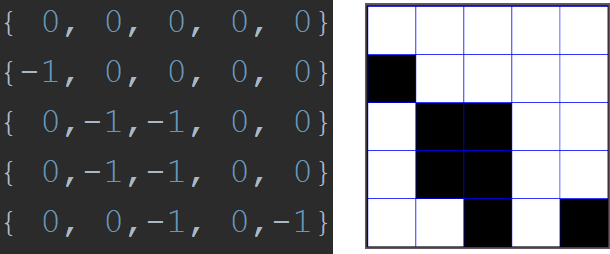
\includegraphics[width={0.5\textwidth}]{laberintom.png}
    \caption{Matriz y su representación mas visual.}
  \end{figure}
  
En este problema las pruebas se realizaron para la matriz anterior.
\newcounter{ct}
\newcounter{n}

% Numero de ejercicios
\setcounter{n}{4}
\stepcounter{n}

\forloop{ct}{1}{\value{ct}<\value{n}}%
{%
  \section*{\mystr\text{ }\arabic{ct}:}
  \subfile{TeXFiles/\enun\arabic{ct}}
  \IfFileExists{Images/\imag\arabic{ct}.png}{
  \begin{figure}[H]
  \centering
    \includegraphics[width={0.5\textwidth}]{\imag\arabic{ct}}
  \end{figure}}{
	  
  }
  \IfFileExists{Images/\imag\arabic{ct}.jpg}{
  \begin{figure}[H]
  \centering
    \includegraphics[width={0.5\textwidth}]{\imag\arabic{ct}}
  \end{figure}}{
	  
  }
  \lstinputlisting[language=Java,linebackgroundcolor={\ifodd\value{lstnumber}\color{claro}\fi}]{Code/\mystr\arabic{ct}.java}
  

 
  	\pagebreak
  
  
  %\pagebreak
  %\includegraphics[scale=0.75]{\mystr\arabic{ct}}
  %\mystr\arabic{ct}
}

%\section*{Anexos}
%Funciones auxiliares para realizar los ejercicios
%\lstinputlisting[language=Java,linebackgroundcolor={\ifodd
%\value{lstnumber}\color{claro}\fi}]{Code/Anexos.java}


\end{document}